\documentclass{article}
\usepackage[utf8]{inputenc}
\usepackage{graphicx}
\title{Portail Library}
\author{Saurabh Agrahari(201416247) and Ashutosh Ranjan(201425031)}
\date{May 2015}

\begin{document}

\maketitle



\section{Brief Description of the Project}



\large{The library maintains info about its books and digital content. Registered users can browse 
    through the available category of books/digital content, access the resource online/request for 
	an issue, get notification/email of due date et cetera. Some of the functions are managed manually by the librarian(admin).}


\section{Features Implemented}
\subsection{Login, Register, Forgot password}
\large{The students and faculty(users) and the admin(librarian) can register easily by filling in the details. Once a student registers(signs up for the first time) the admin categorizes the user as faculty or student manually. Only after that the user is able to use the resources of the portal. A registered user can also change the password if he/she has forgotten it by the "Lost Password" feature.}

\subsection{Adding books to the database}
\large{The admin can add books to the database anytime he wishes by filling in the details. This feature is priviledged and can be accessed only by the admin.}

\subsection{Searching and Issuing books}
\large{Any user/admin can search the database for books even if he/she hasn't registered/logged in yet. However to issue the book he/she has to login.}

\section{Features that need more work}
\subsection{Email sending}
\large{The admin should be able to send emails to the users who have borrowed the books and also send the details about the fine due. This feature hasn't still been implemented perfectly and needs work.}
\section{Schema of tables used}
\large{Table with name "BOOKS" stores all the books in the database. Table with name "Issue" and "Register" stores all the issued books and the names of registered users respectively.}  

\newpage
\section{UI Screenshots}

\begin{figure}[ht!]
\centering
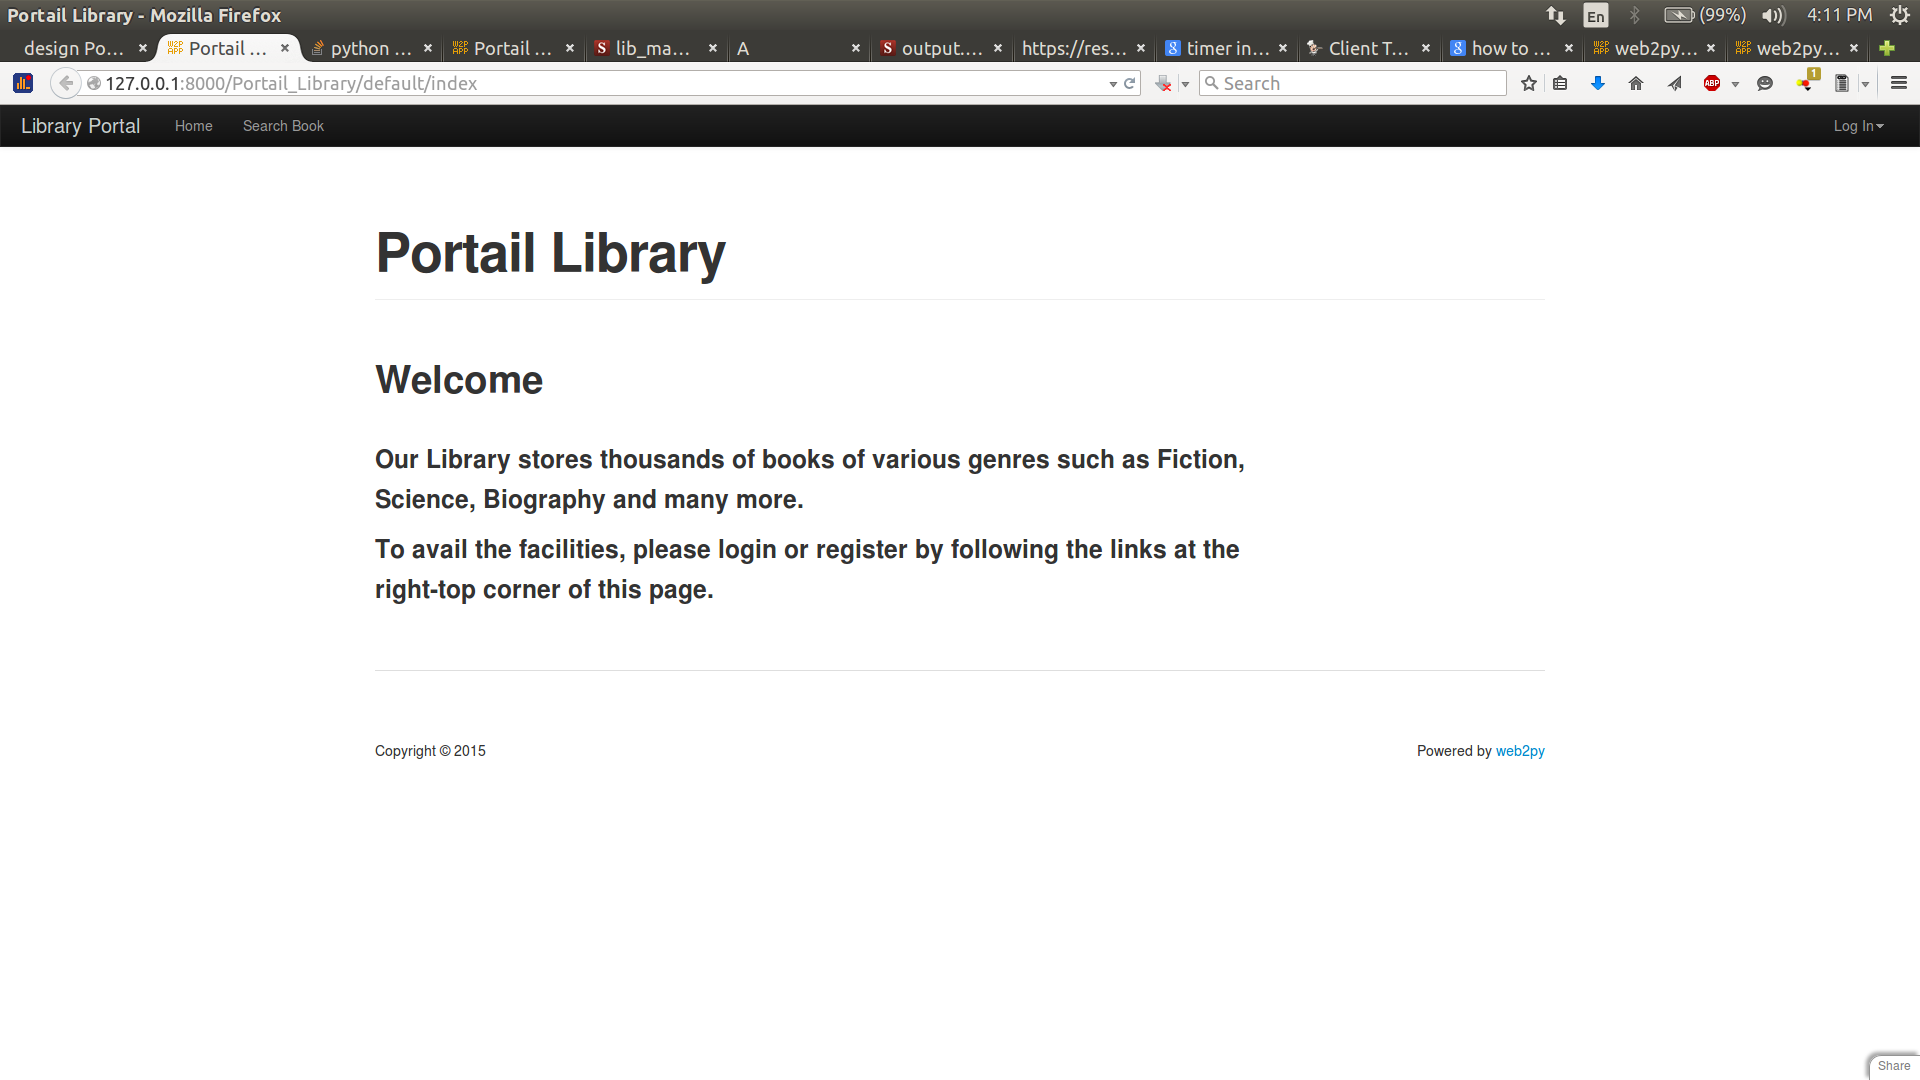
\includegraphics[width=100mm]{1.png}
\caption{}
\end{figure}
\begin{figure}[ht!]
\centering
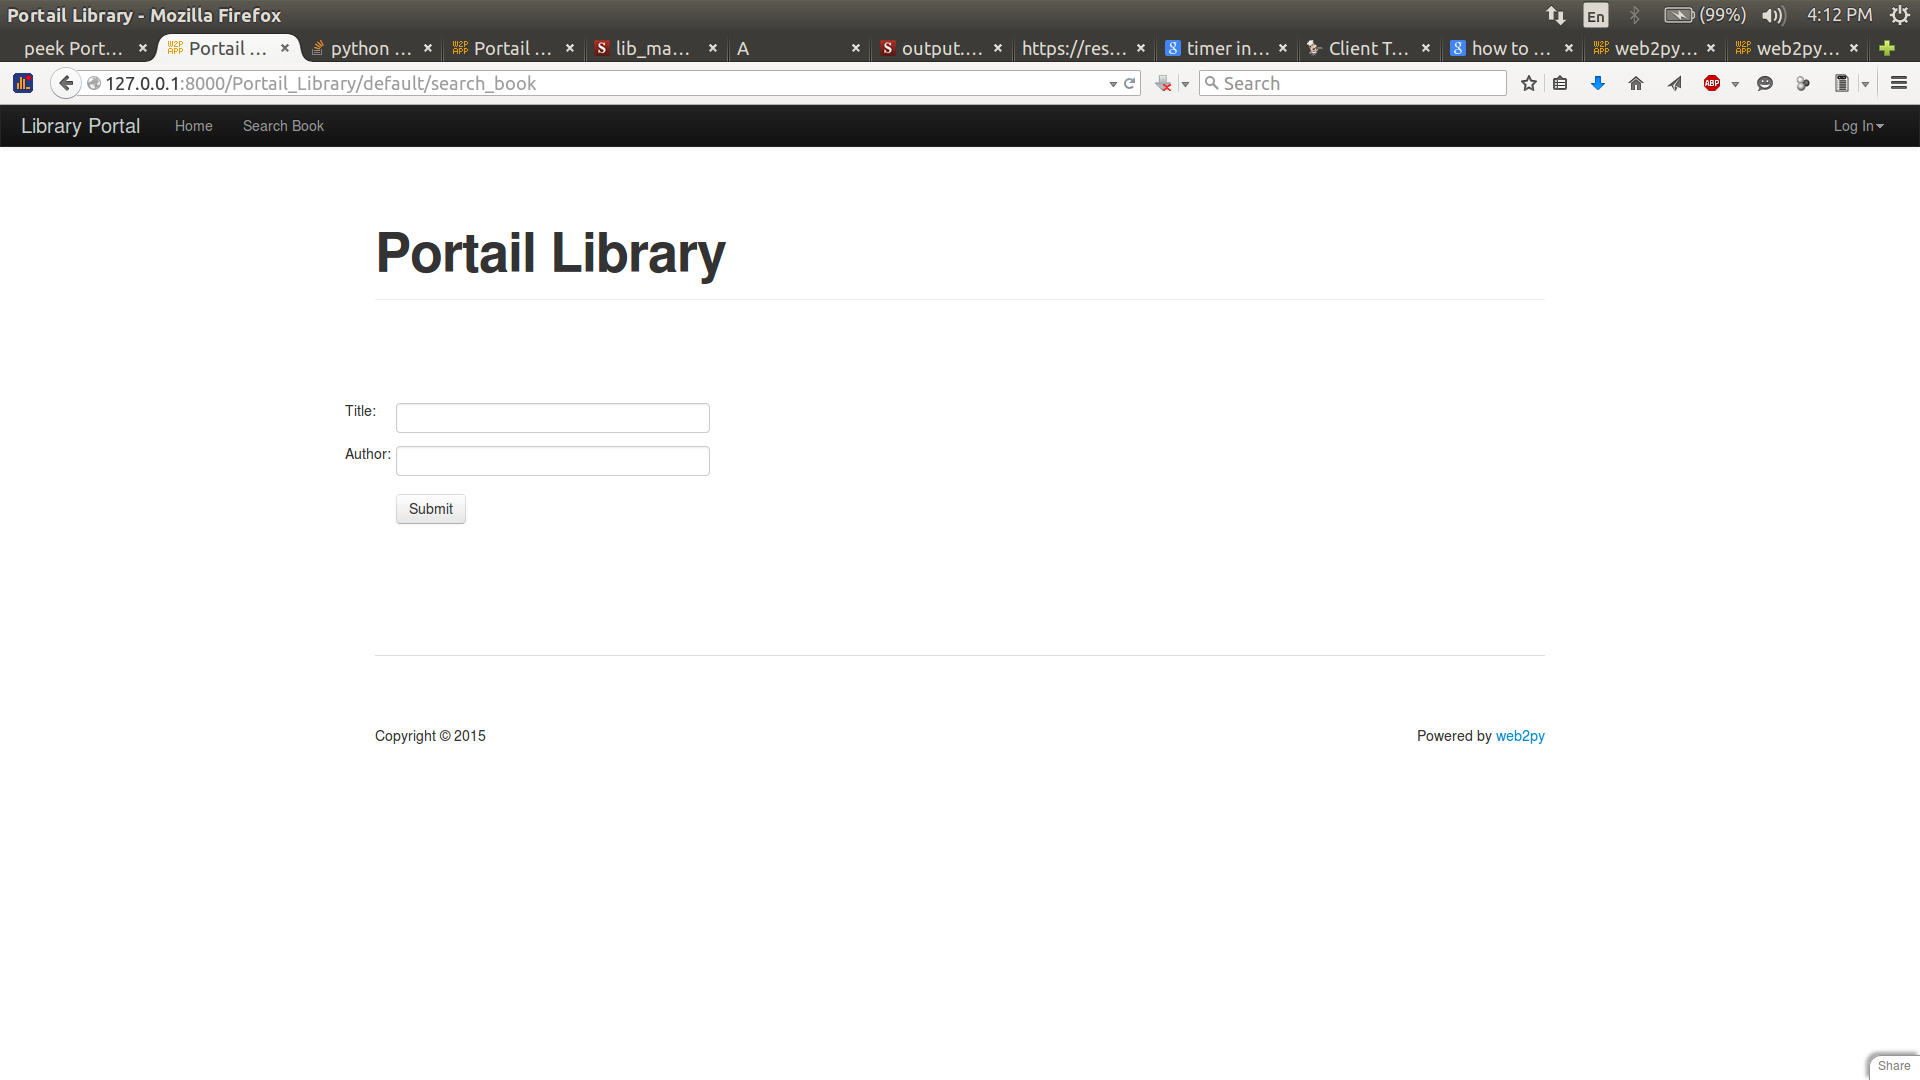
\includegraphics[width=100mm]{2.png}
\caption{}
\end{figure}
\begin{figure}[ht!]
\centering
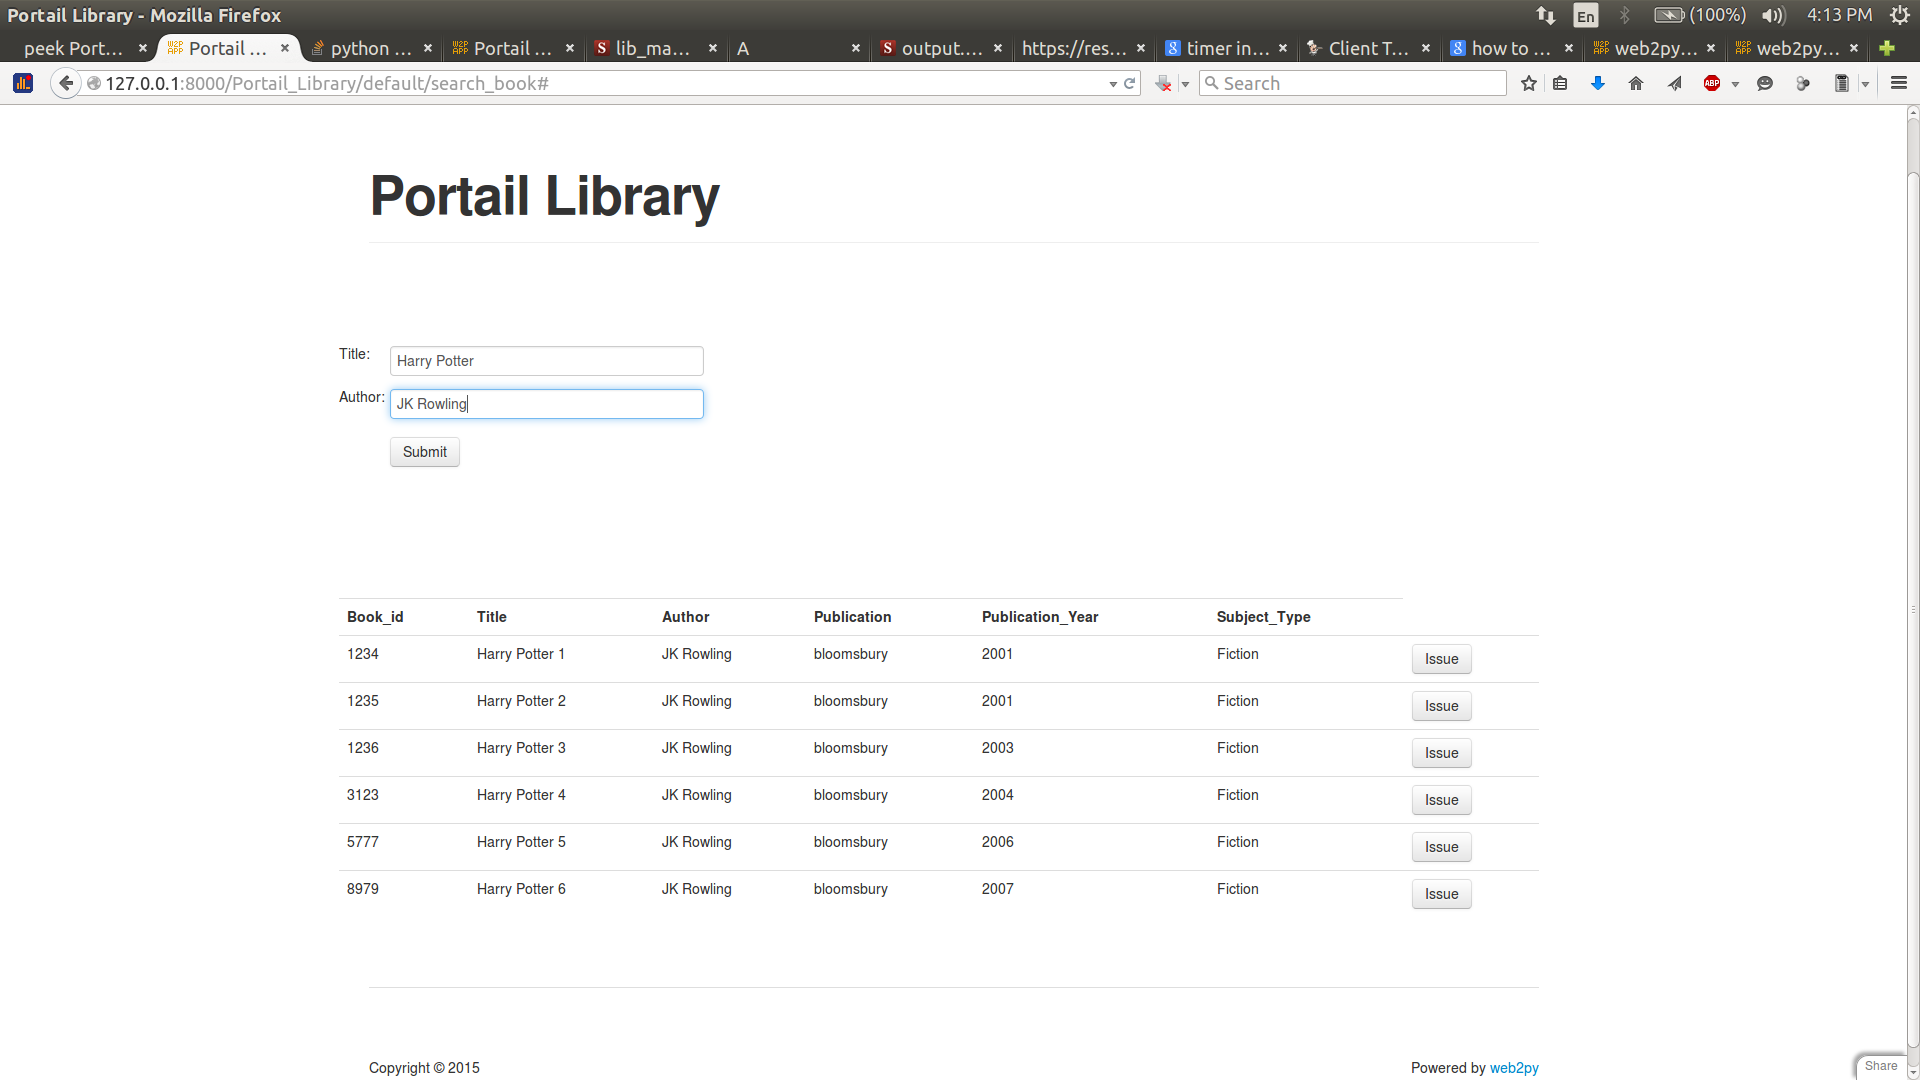
\includegraphics[width=100mm]{3.png}
\caption{}
\end{figure}
\begin{figure}[ht!]
\centering
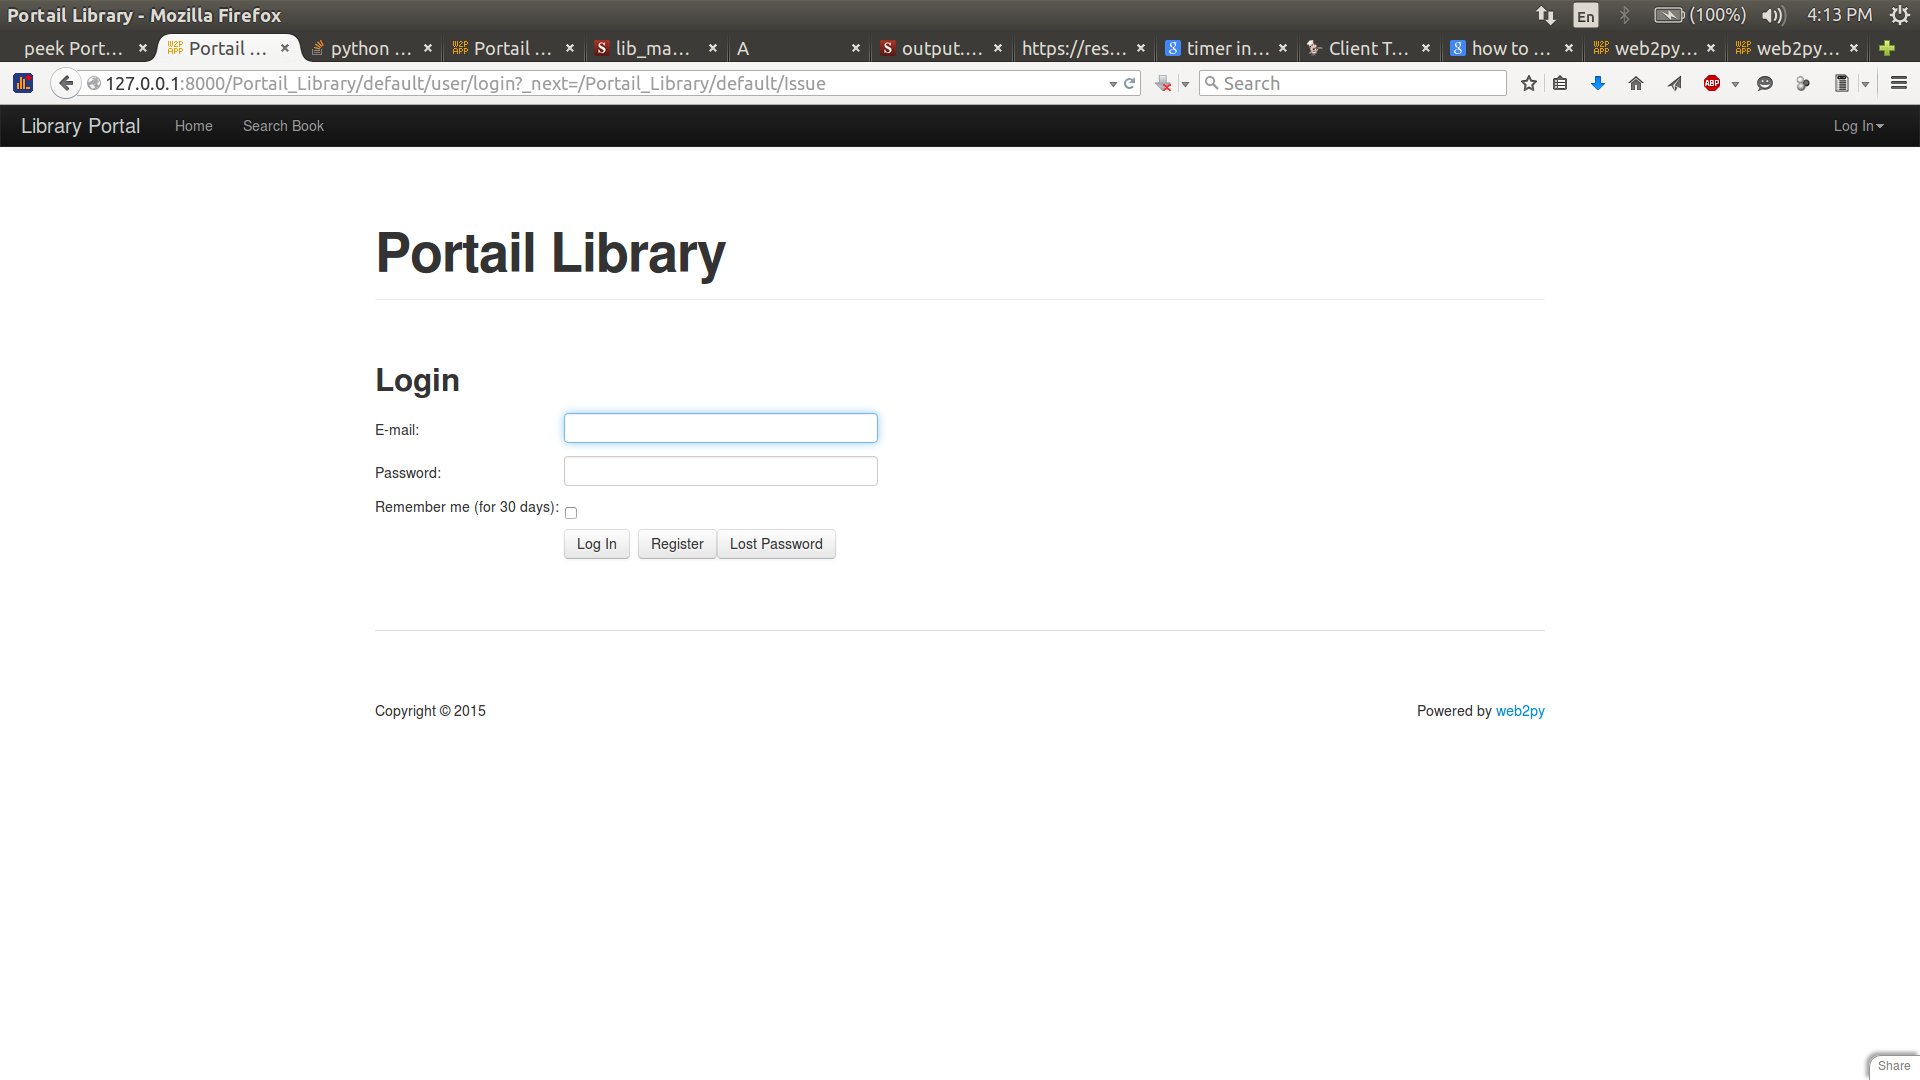
\includegraphics[width=100mm]{4.png}
\caption{}
\end{figure}
\begin{figure}[ht!]
\centering
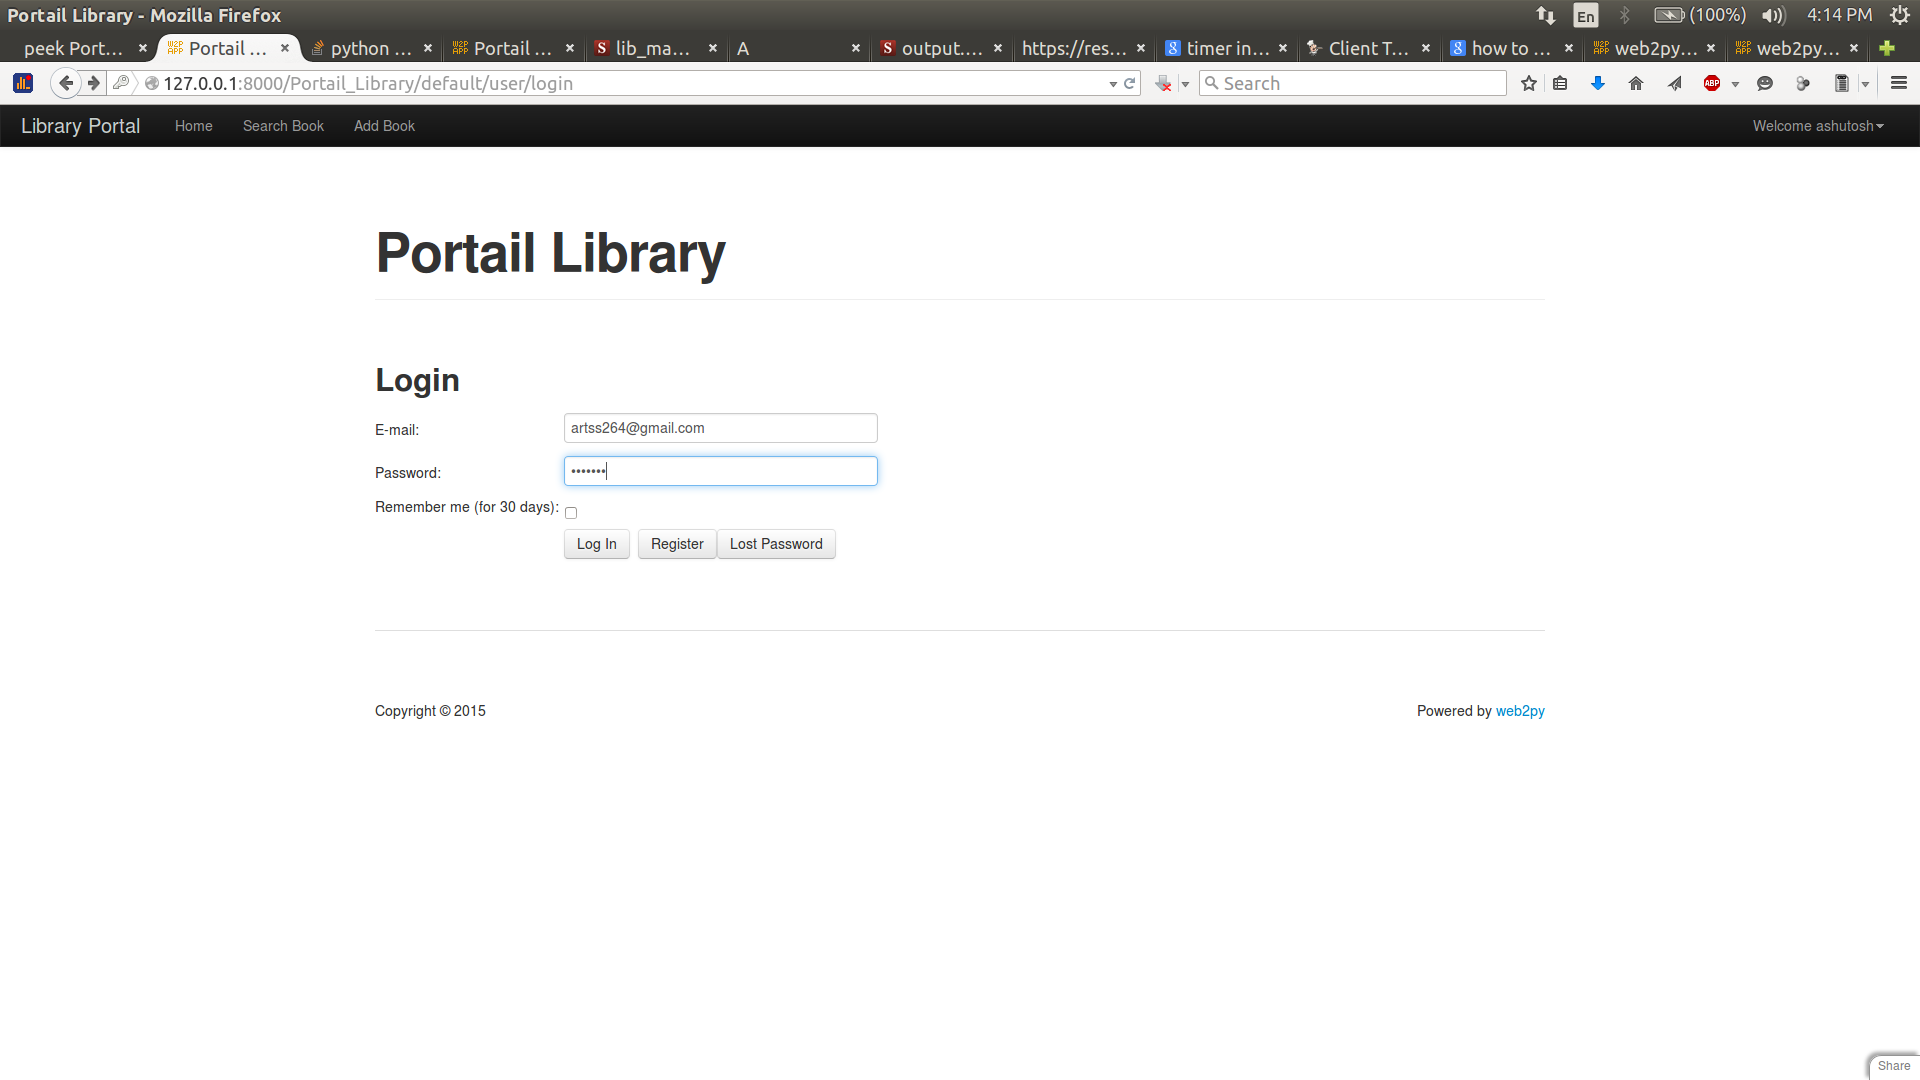
\includegraphics[width=100mm]{5.png}
\caption{}
\end{figure}
\begin{figure}[ht!]
\centering
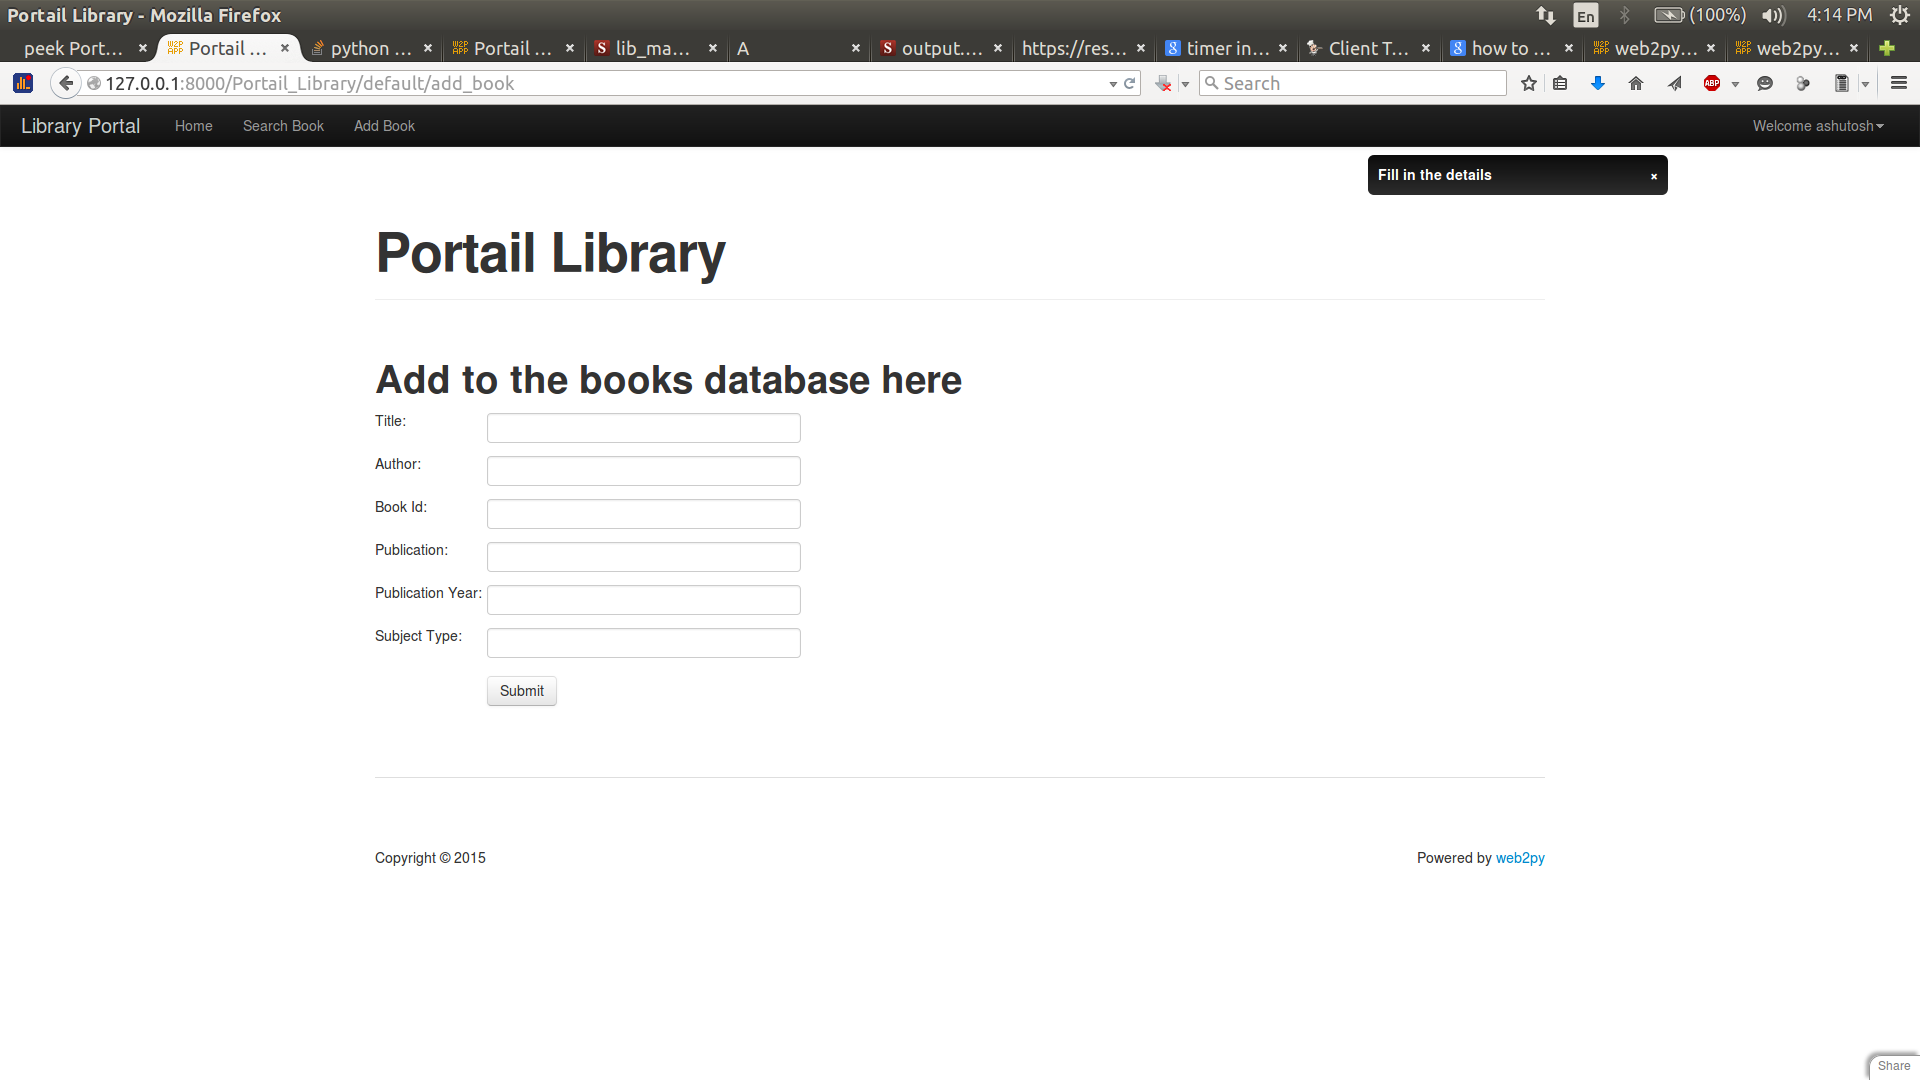
\includegraphics[width=100mm]{6.png}
\caption{}
\end{figure}
\begin{figure}[ht!]
\centering
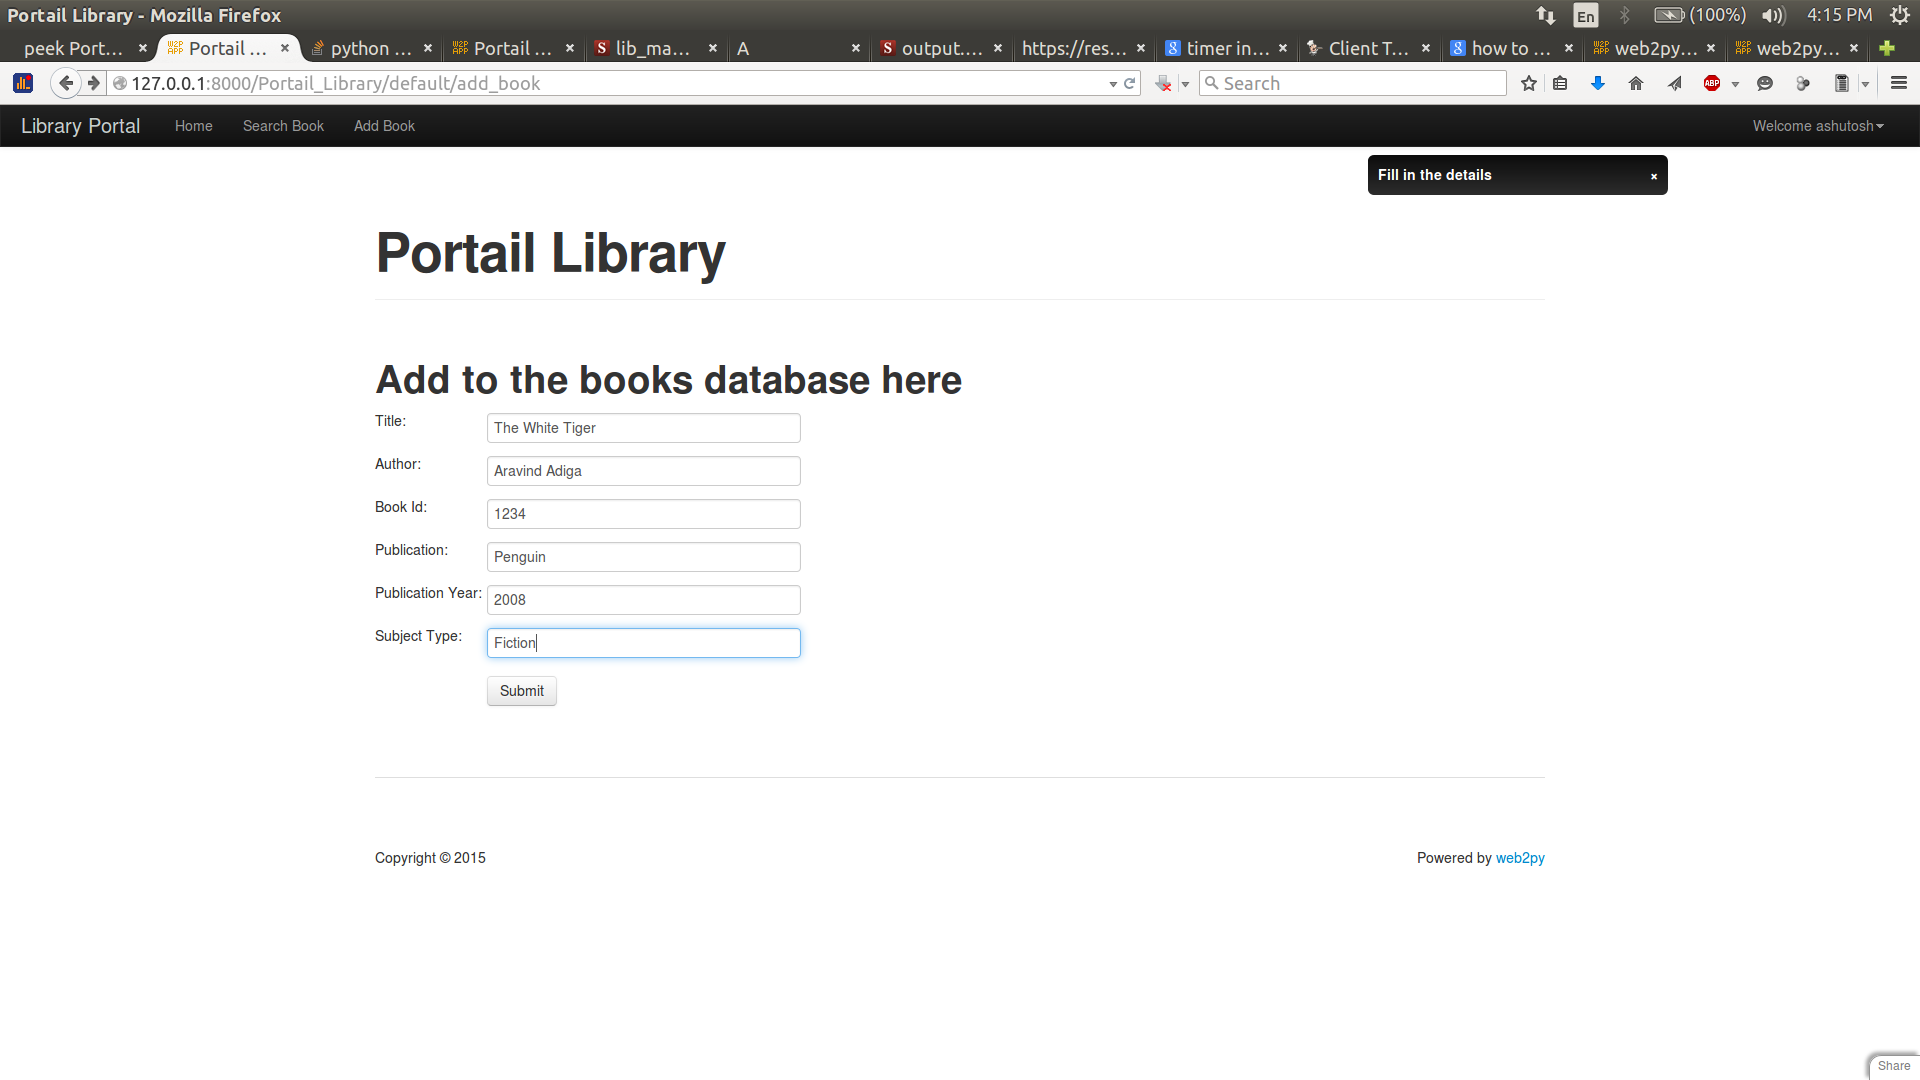
\includegraphics[width=100mm]{7.png}
\caption{}
\end{figure}
\begin{figure}[ht!]
\centering
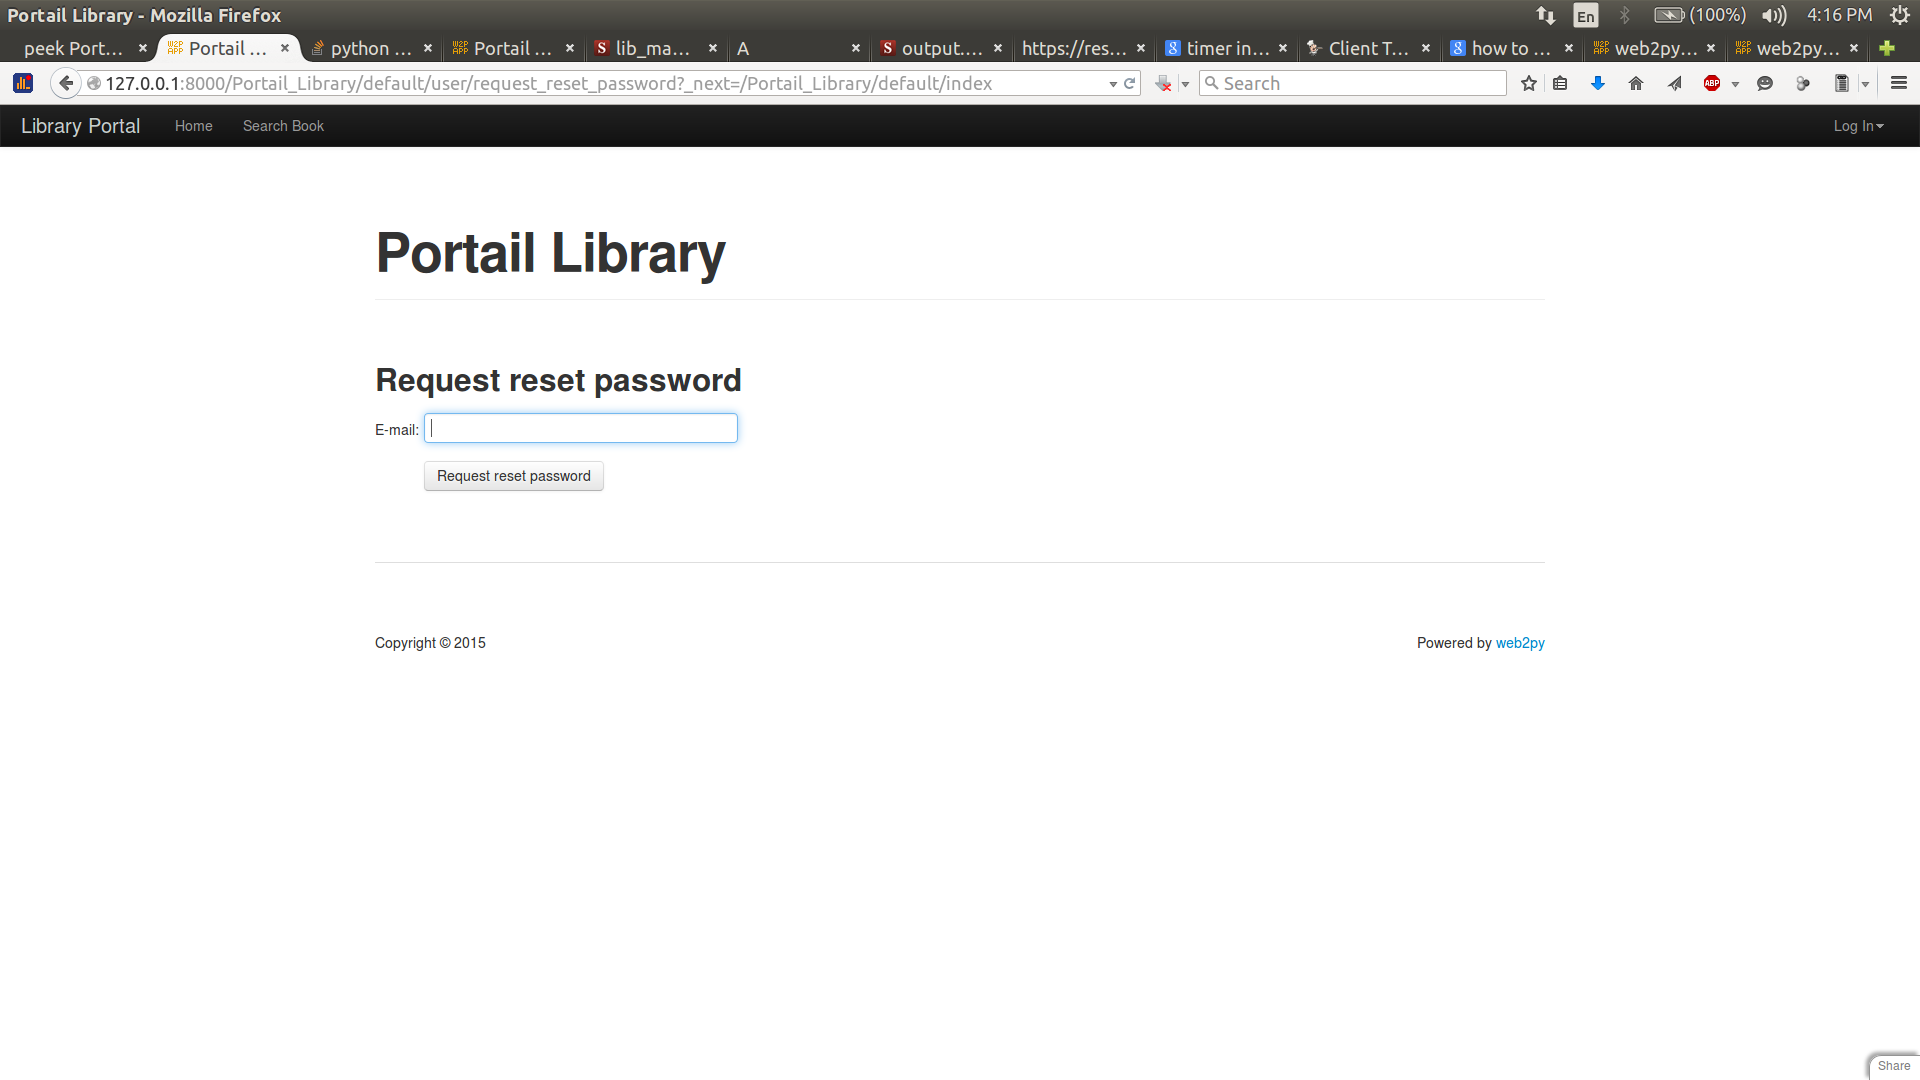
\includegraphics[width=100mm]{8.png}
\caption{}
\end{figure}
\begin{figure}[ht!]
\centering
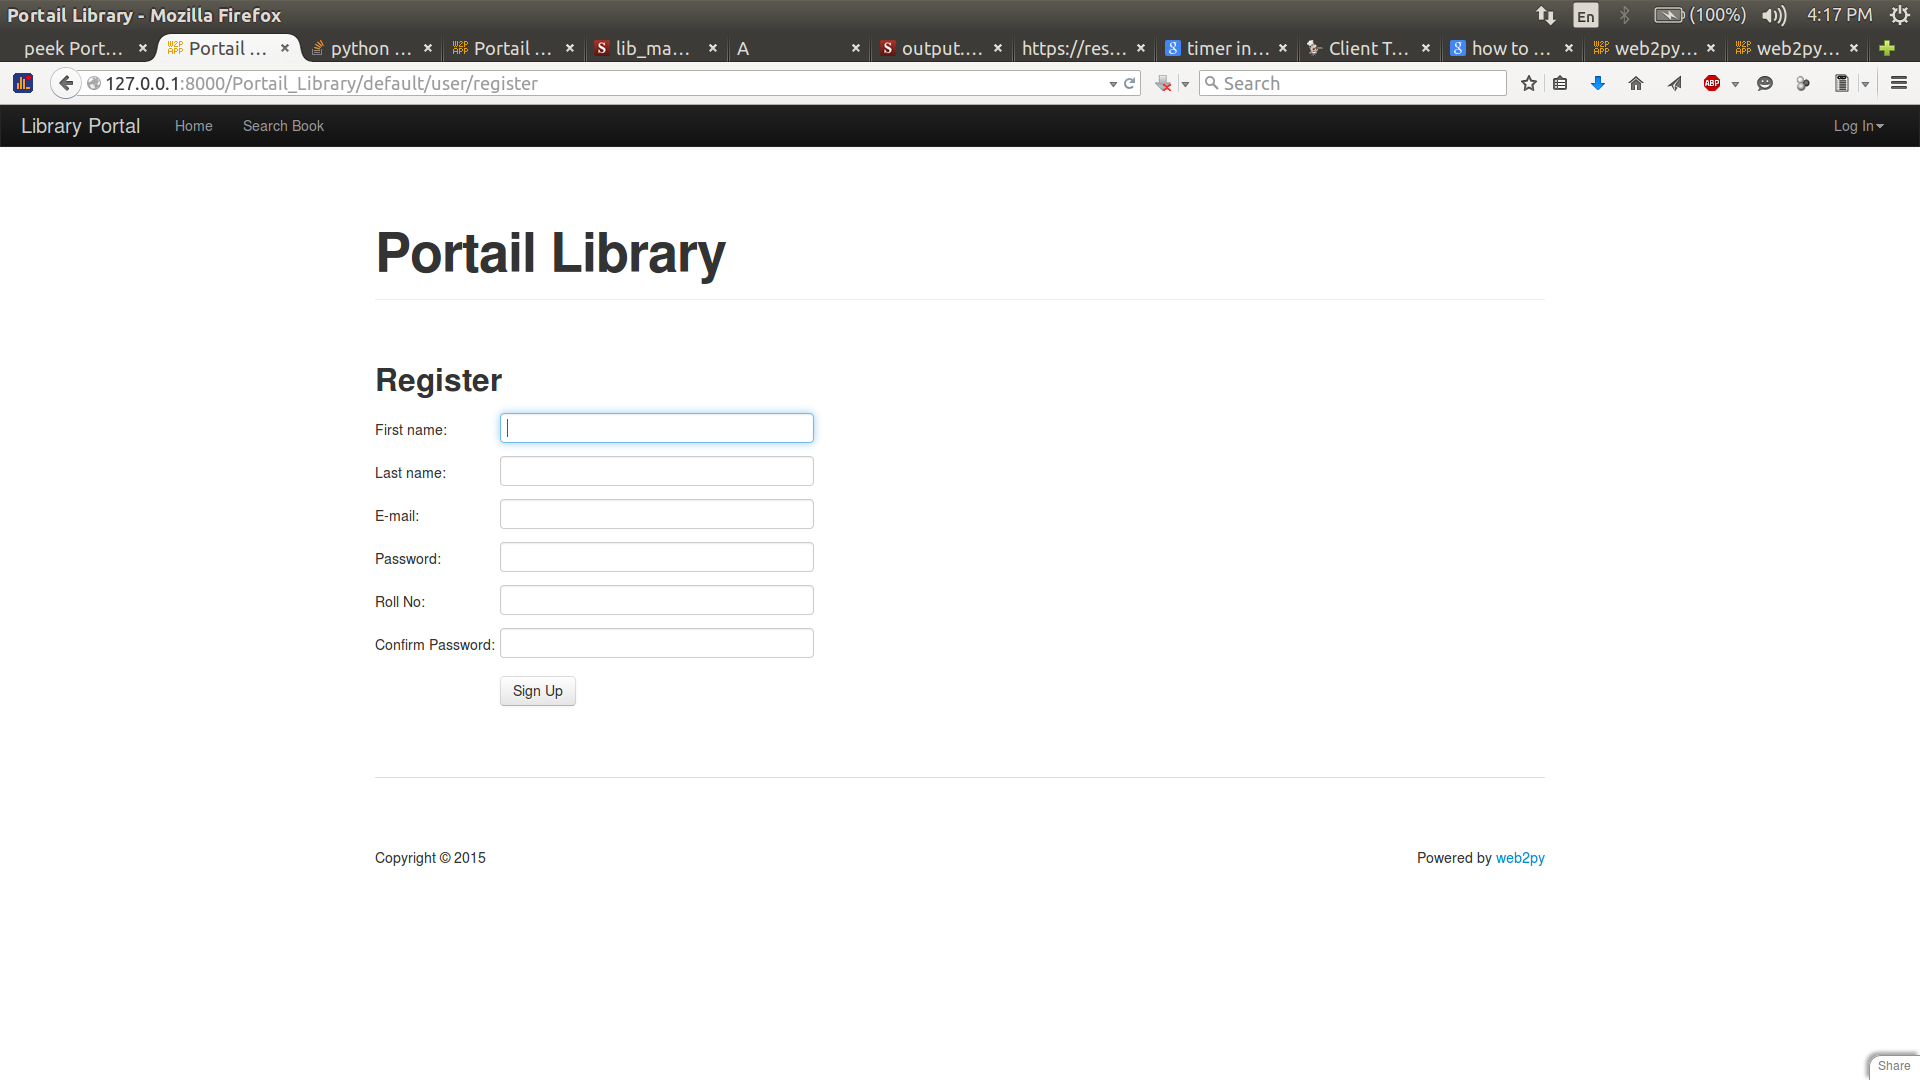
\includegraphics[width=100mm]{9.png}
\caption{}
\end{figure}
\begin{figure}[ht!]
\centering
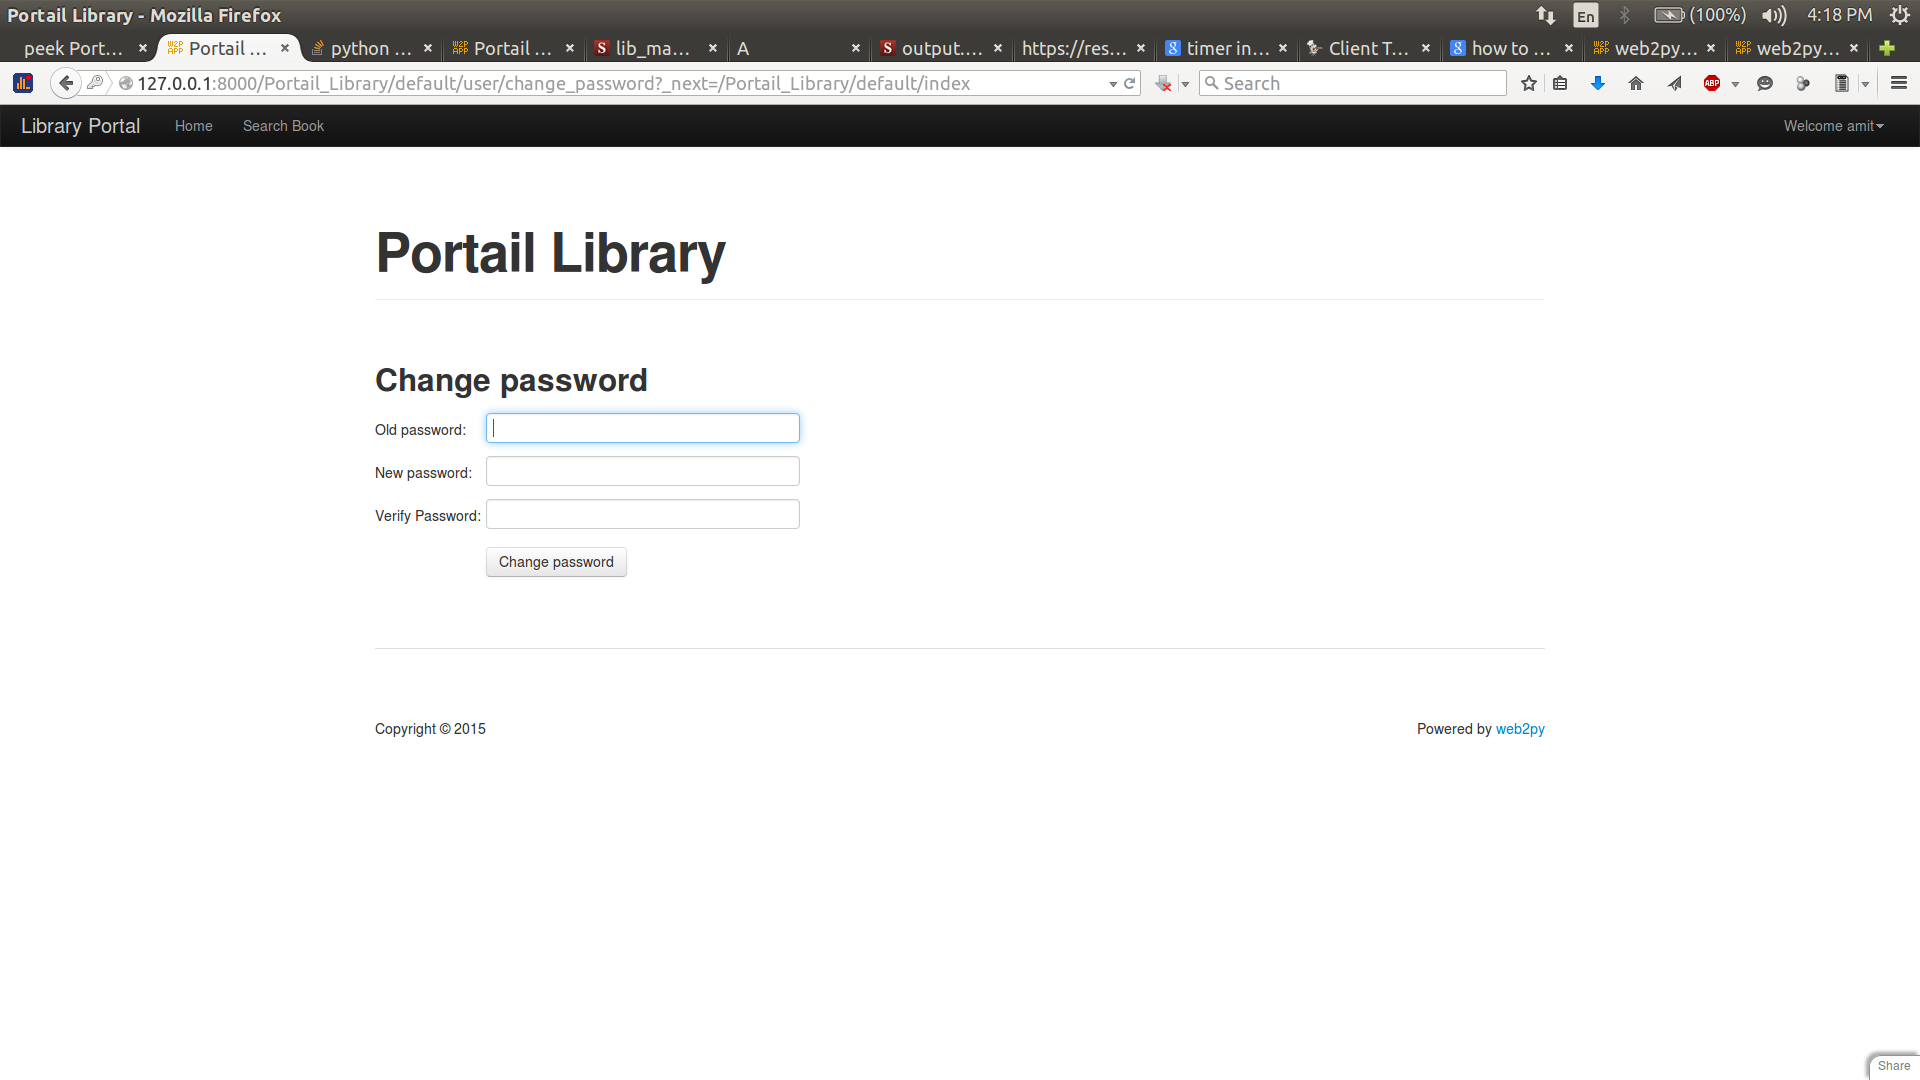
\includegraphics[width=100mm]{10.png}
\caption{}
\end{figure}
\begin{figure}[ht!]
\centering
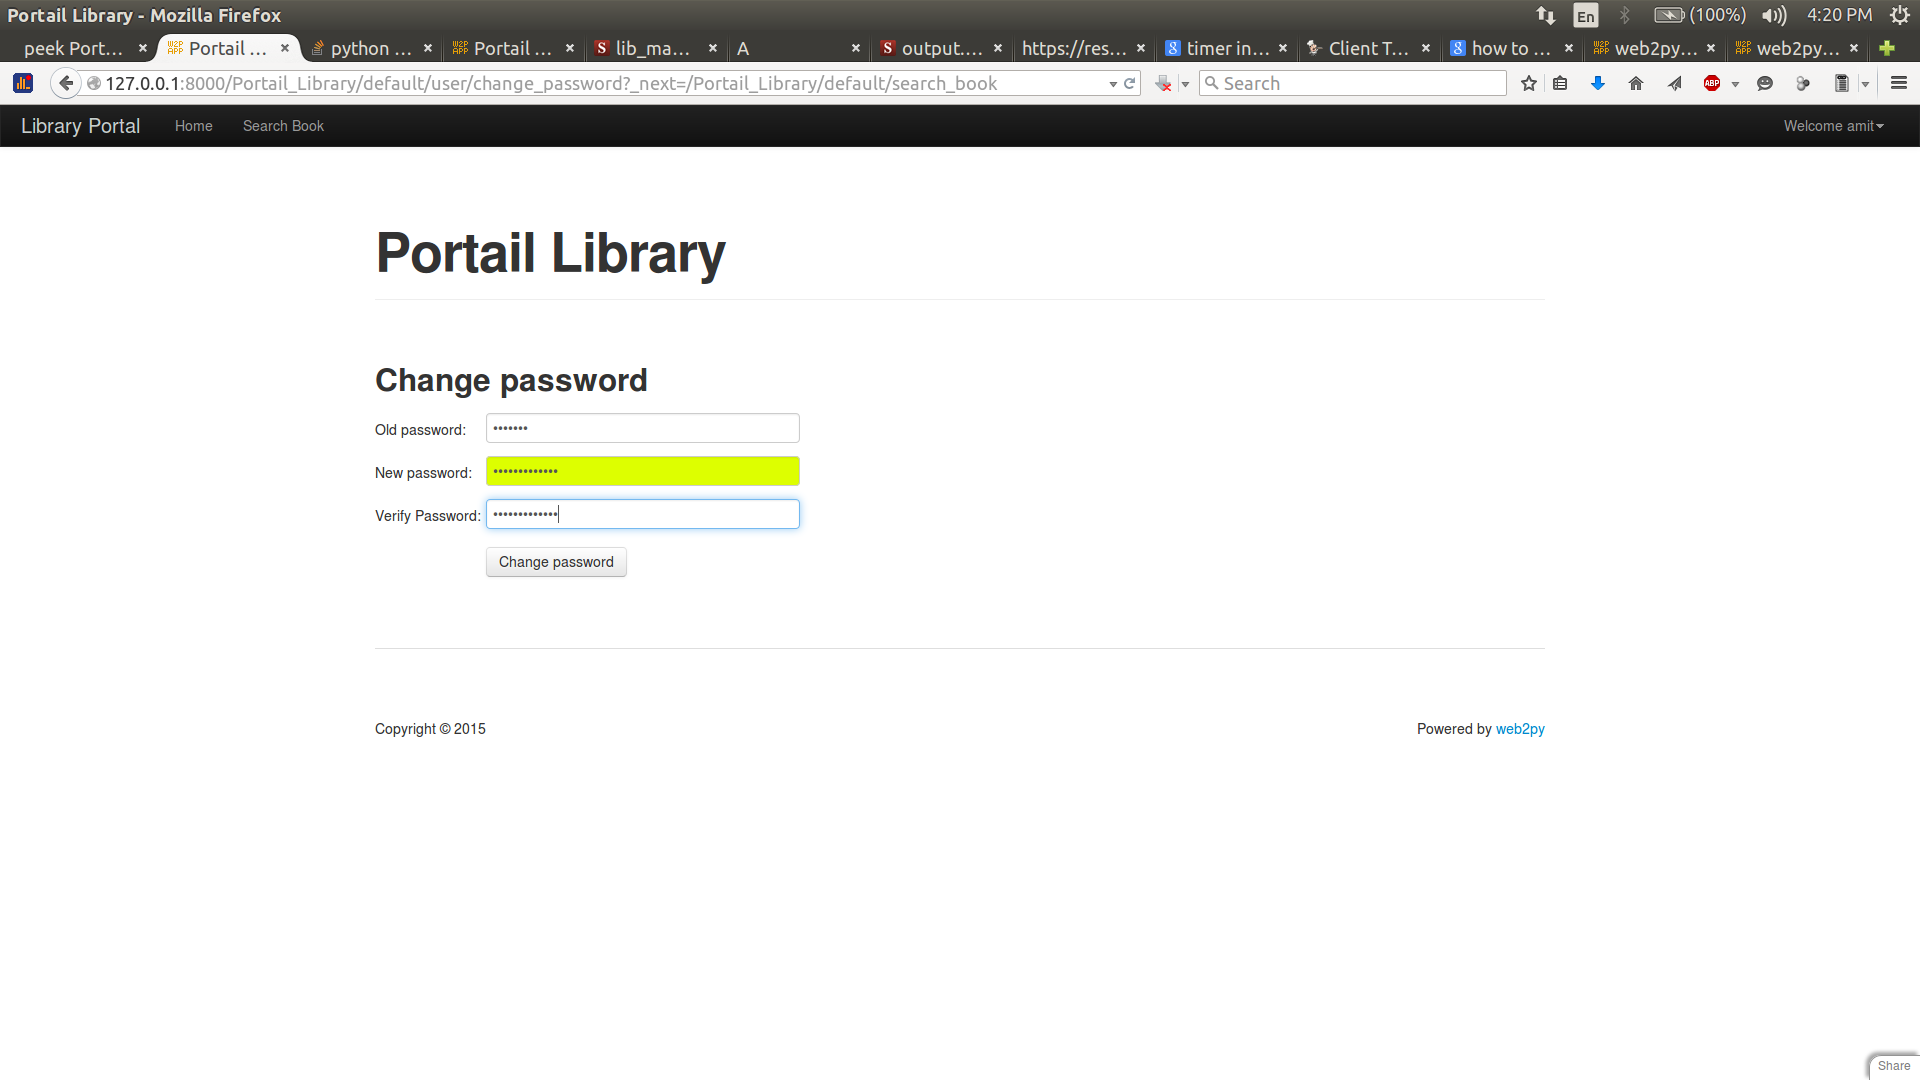
\includegraphics[width=100mm]{11.png}
\caption{}
\end{figure}
\begin{figure}[ht!]
\centering
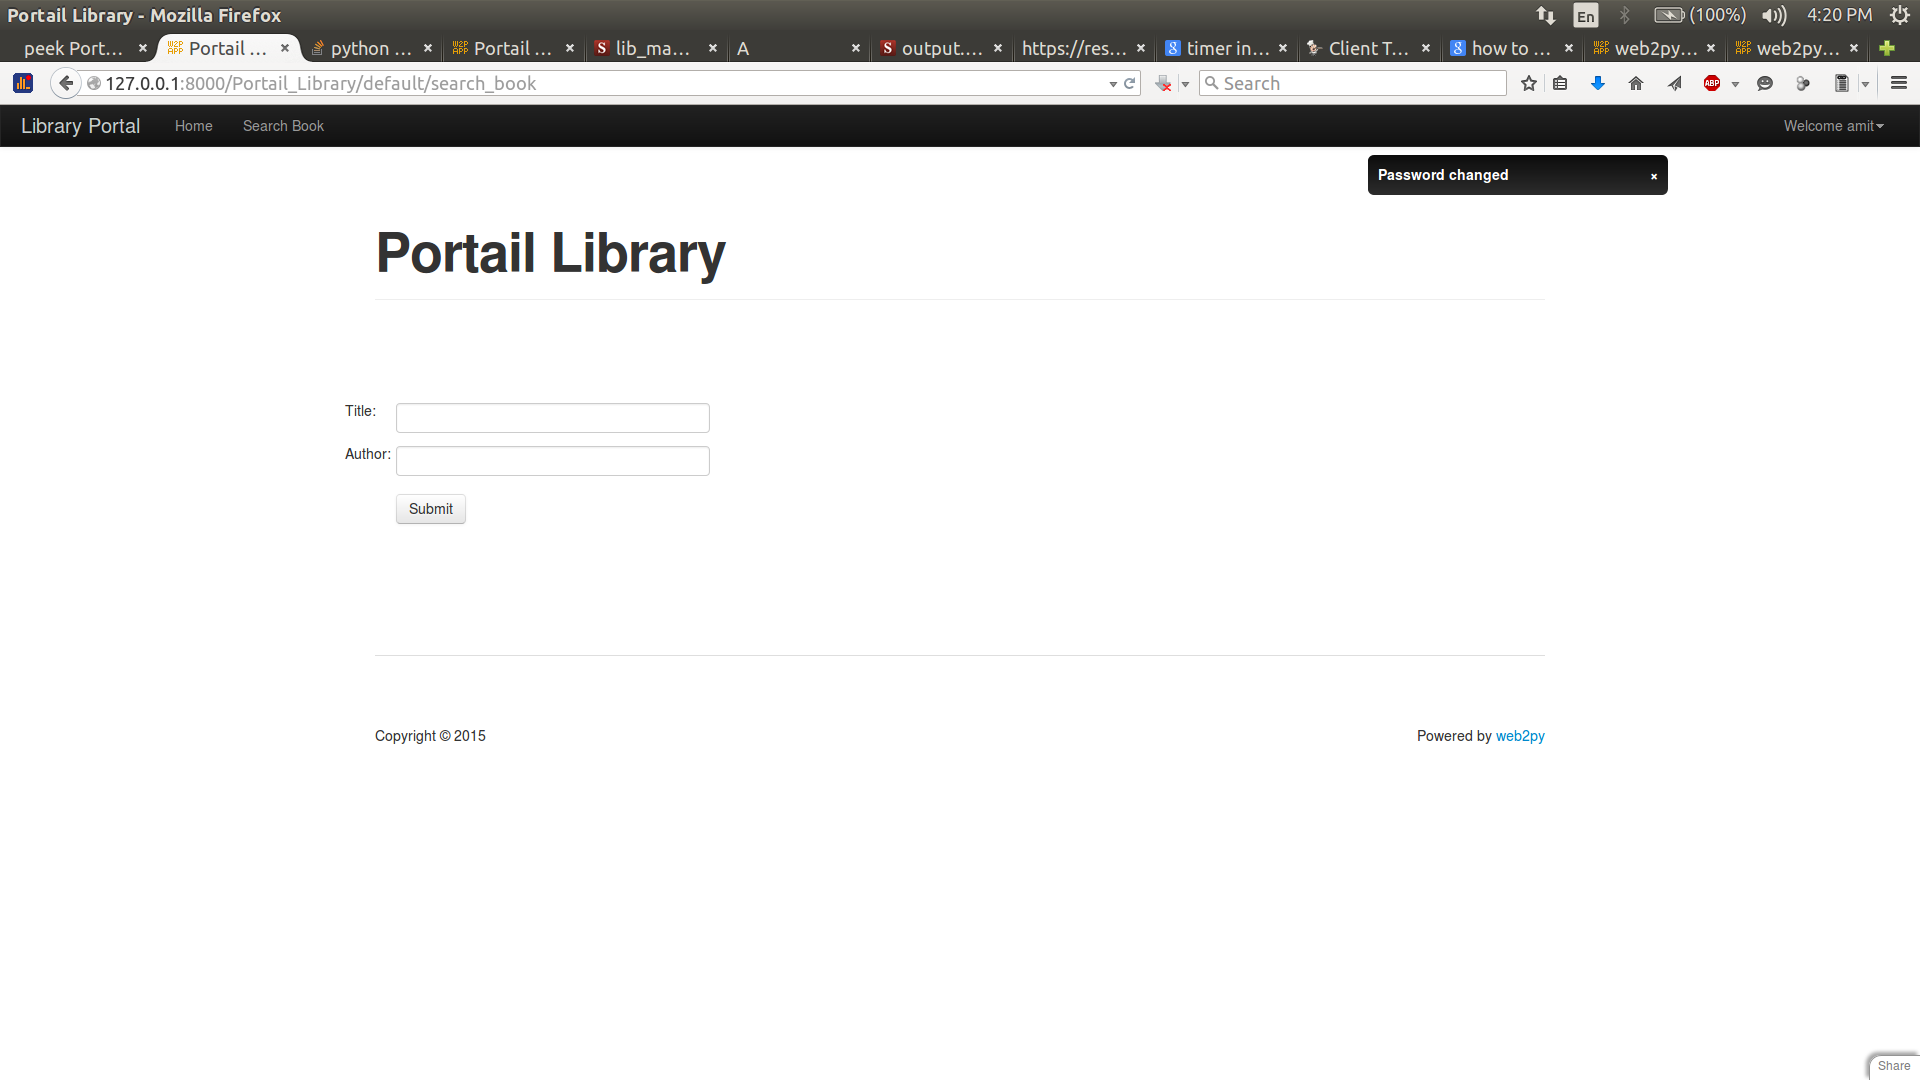
\includegraphics[width=100mm]{12.png}
\caption{}
\end{figure}
\newpage
\end{document}

